\section{Floyd$-$Warshall}\label{sec:fw}
\subsection{Implementation}
The algorithm implemented in the original code runs in $O(\log(N)N^3)$ while
Floyd$-$Warshall runs in $O(N^3)$. This means in theory that Floyd-Warshall
should be significantly faster than the original code. Floyd$-$Warshall is very
similar to the original code, except the loop order is $kij$ (or $kji$), As we
must calculate the shortest distance using all nodes less than or equal to the
current $k$ before calculating for $k+1$. This means the entire set of 3 nested
loops cannot be parallelized. Instead only the inner two can. This decreases
the amount of parallelism and increases the frequency with which data must be
synchronized, while decreasing overall work. We implemented Floyd$-$Warshall (a
rather simple set of changes to the original implementation) in both OMP and
MPI. Our implementations are in \texttt{fw-omp.c} and \texttt{fw-mpi.c}
respectively.

\subsection{Performance}
\begin{figure}[h]
  \centering
  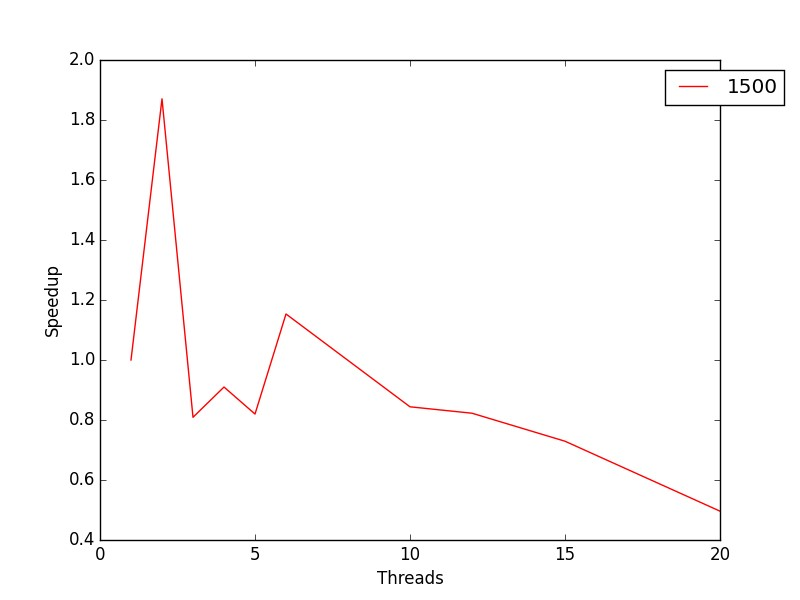
\includegraphics[width=0.68\textwidth] {plots/6}
  \caption{%
    Strong scaling speedup of our Floyd$-$Warshall MPI code as number of MPI
    ranks increases. Baseline for calculating speedup is Floyd-Warshall MPI
    code with 1 rank.
  }
  \label{aload0}
\end{figure}
\begin{figure}[h]
  \centering
  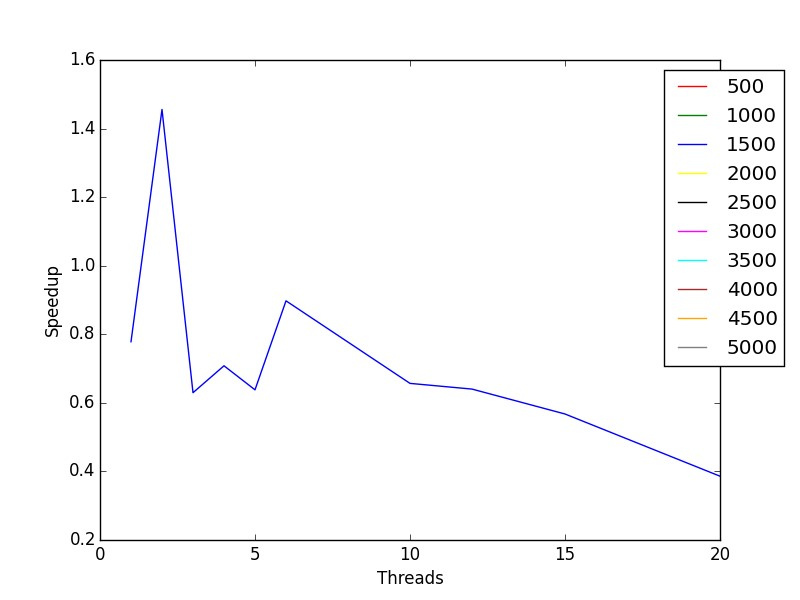
\includegraphics[width=0.68\textwidth] {plots/7}
  \caption{%
    Strong scaling speedup of our Floyd$-$Warshall MPI code as number of MPI
    ranks increases. Baseline for calculating speedup is our original MPI code
    with 1 rank.
  }
  \label{aload1}
\end{figure}

We tested our Floyd$-$Warshall code for a single $n$ (1500), as it does not
scale well. We calculated strong scaling for this $n$ using a baseline of the
Floyd$-$Warshall MPI code with 1 rank (Figure 6) and a baseline of our original
MPI code with 1 rank (Figure 7). In Figure 6, the performance of FW MPI
increases only until 2 and then starts to drop off. This is for two reasons:
the first is the increased overhead once we go beyond 12 ranks (communication
across 2 chips is slower) and the larger reason is that communication is
expensive in Floyd$-$Warshall. Because we have to synchronize $O(N)$ times
rather than $O(\log(N))$ times as we increase the amount of communication that
is done (by increasing number of ranks) we see that our code gets slower as we
add more parallelism.

In Figure 7 we can see that our speedup is even smaller when compared to our
original MPI code, for the exact same reason as before: The extra communication
is a major cost and results in a decline in performance as rank increases.
